\title{\textbf{A Robust Localization Scheme for Interpolation of Unstructured Grids}}
\author{
        Rajiv Shenoy \\
        Georgia Institute of Technology\\
        Mentor: Dr. Michael Park\\
        Research and Technology Directorate � CASB D302\\
}
\date{\today}

\documentclass[12pt]{article}
\usepackage[top=1.0in, bottom=1.0in, left=1.5in, right=1.0in]{geometry}
%\usepackage{apacite}
\usepackage{graphicx,color}
\usepackage{subfigure,subfig}

\graphicspath{{Figures/}}

%\makeatletter
%\newenvironment{tablehere}
%{\def\ @captype{table}}
%{}
\newenvironment{figurehere}
{\def\ @captype{figure}}
{}
%\makeatother

\begin{document}
\maketitle

\begin{abstract}
This is the paper's abstract \ldots
\end{abstract}

\newpage
\section{Introduction}
Due to recent advances in the computational capability for computational fluid dynamics (CFD) simulations, typical problems require parallel computing power involving a large number of processors. Therefore, it becomes imperative for developers to optimize codes for efficiency of any process during a simulation and ensure parallel scalability. Feature or adjoint-based grid adaptation may be utilized in a time-dependent simulation to increase accuracy. Any subsequent grid modifications require a solution transfer of the current time step and those of backplanes from the background grid to the new grid. In order to ensure an accurate solution transfer, trilinear interpolation, which ensures $2^{nd}$ order accuracy is a requisite. A further increase in accuracy may be achieved using a conservative interpolation scheme. A major impediment of an accurate interpolation scheme is the ability to efficiently localize nodes of the new grid to the enclosing elements of the background grid.
	NASA�s state of the art unstructured code, FUN3D, currently employs an interpolation scheme that does not fulfill the requisite accuracy for a time-accurate simulation. The simple brute force search algorithm for enclosing elements could approach prohibitive limits for high end grids resulting in $O(n^{2})$ searches. Load balancing of the adapted grid will complexify the parallel search algorithm. Therefore, a novel approach is proposed in the present effort involving a sweeping scheme that would robustly expedite localization. An advancing front scheme using neighbor walks to speed up searches is employed from relevant literature. Such a scheme has shown promise on serial applications to minimize the number of searches. In order to overcome special situations such as searches across a geometric boundary in a concave domain, a hierarchical approach is proposed, wherein the localization is initiated at boundary corners and then progressing into boundary edges, surfaces, and finally advancing into the volume.
	Preliminary results have realized the minimization of searches using the serial advancing front scheme. The parallel implementation is expected to scale with processors and result in $O(n)$ searches. Tabulated results will be presented to detail the benefits in both CPU time and number of searches. Test cases involving adaptive static and moving grid systems will be utilized to assess performance improvements. In addition to solution transfers for grid adaptation, the proposed localization scheme should provide benefits to other CFD related concerns such as grid sequencing and for overset grid interpolation.
	
% Need to talk about Loehner and Alauzet

% Noack + Djomehri et al.

\section{Approach}

\subsection{Neighbor Walk}

\begin{figurehere}
\begin{center}
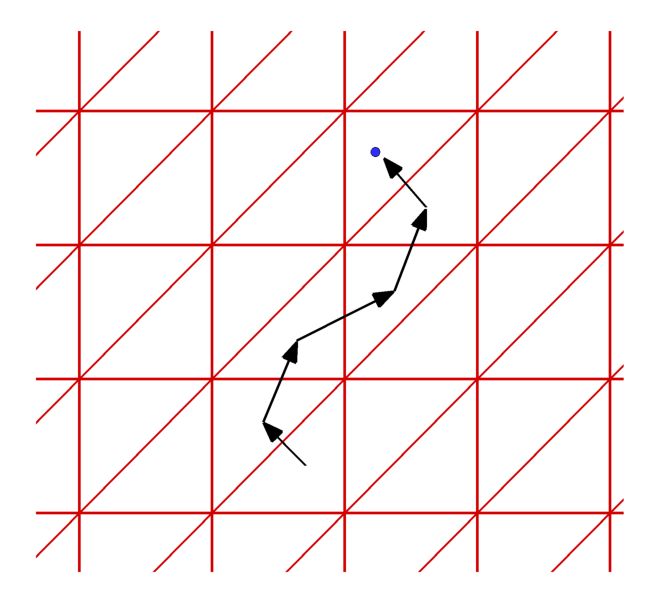
\includegraphics[trim = 0.0cm 0.0cm 0.0cm 0.0cm, clip, width=0.5\textwidth]{neighbor_walk.png}
\label{fig:neighbor_walk}
\end{center}
\end{figurehere}

\subsection{Advancing Front}

\begin{figurehere}
\begin{center}
  \subfigure[Seeding]{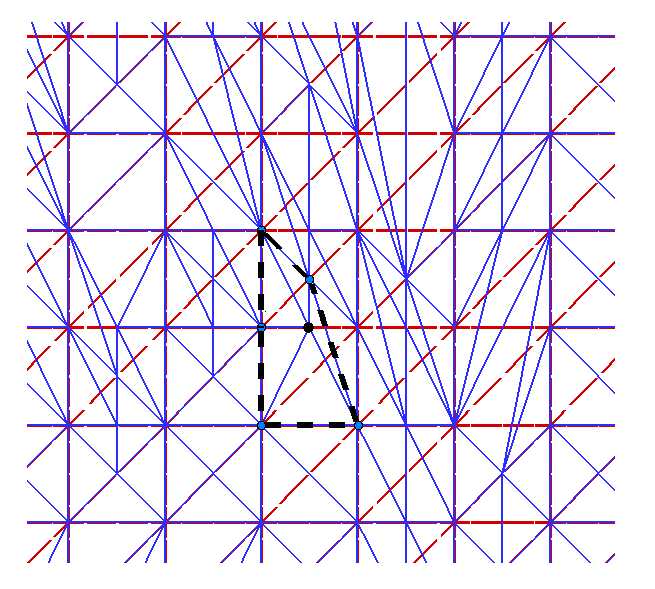
\includegraphics[trim = 0.0cm 0.0cm 0.0cm 0.0cm, clip, width=0.3\textwidth]{advancing_front_1.png}} 
  \subfigure[Front Advancement]{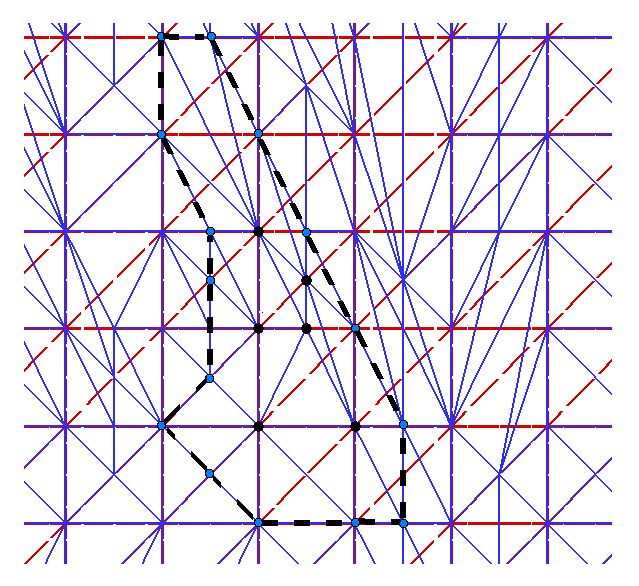
\includegraphics[trim = 0.0cm 0.0cm 0.0cm 0.0cm, clip, width=0.3\textwidth]{advancing_front_2.png}}
\label{fig:neighbor_walk}
\end{center}
\end{figurehere}

\subsection{Parallel Paradigm}

\section{Results}

% Efficiency tests on Box Grid

% Time Accurate Adaptation on Moving Grid

\section{Future Work}

\section{Conclusion}


\begin{thebibliography}{30}
%\bibliographystyle{apacite}
\bibitem{alauzet_mehrenberger}
Alauzet, F. and Mehrenberger, M., "$P^{1}$-Conservative Solution Interpolation on Unstructured Triangular Meshes", {\it International Journal of Numerical Methods in Engineering}, Vol.~84,~(13), pp.1552-1588, 2010.

\bibitem{loehner}
L\"{o}hner, R., "Robust, Vectorized Search Algorithms for Interpolation on Unstructured Grids", {\it Journal of Computational Physics}, Vol.~118,~(2), pp.380-387, 1995.

\bibitem{mavriplis}
Mavriplis, D.J., "Multigrid Techniques for Unstructured Meshes", {\it 26th Computational Fluid Dynamics Lecture Series Program of the von Karman Institute (VKI) for Fluid Dynamics}, Rhode-Saint-Gen\`{e}se, Belgium, March, 1995.

\bibitem{loeher_ambrosiano}
L\"{o}hner, R. and Ambrosiano, J., "A Vectorized Particle Tracer for Unstructured Grids," {\it Journal of Computational Physics}, Vol.~91,~(1), pp.22-31, 1990.

\bibitem{noack}
Noack, R.W., "Resolution Appropriate Overset Grid Assembly for Structured and Unstructured Grids," {\it Proceedings of the 16th AIAA Computational Fluid Dynamics Converence}, Orlando, FL, June, 2003.

\bibitem{djomehrietal}
Djomehri, M.J., Biswas, R., Potsdam, M., and Strawn, R.C., "An Analysis of Performance Enchancement Techniques for Overset Grid Applications", {\it International Parallel and Distributed Processing Symposium}, Nice, France, April, 2003.

\end{thebibliography}

\end{document}
